\section{Tendencias temporales}
Se analizaron los 485 meses completos de enero de 1981 a diciembre de 2022.
Para separar la estacionalidad del cambio de largo plazo se usaron anomalías
mensuales: a cada valor se le resta la media histórica de su mes calendario.
Por eso una anomalía positiva significa que el mes estuvo por encima de lo
habitual para ese mes, no que el valor absoluto sea necesariamente alto.

La línea de la figura es una regresión OLS sobre las anomalías. Como resumen
robusto se calculó la pendiente de Sen estacional, comparando únicamente meses
del mismo calendario (eneros entre sí, febreros entre sí, etc.). Mann--Kendall
estacional contrasta una tendencia monotónica; se reporta p bilateral y se toma
$p<0.05$ como evidencia al nivel 5\%. Estos análisis no prueban causalidad ni
resuelven autocorrelación, cambios de estación, regulación, uso del suelo o
falta de homogeneidad del registro.

\begin{figure}[H]\centering
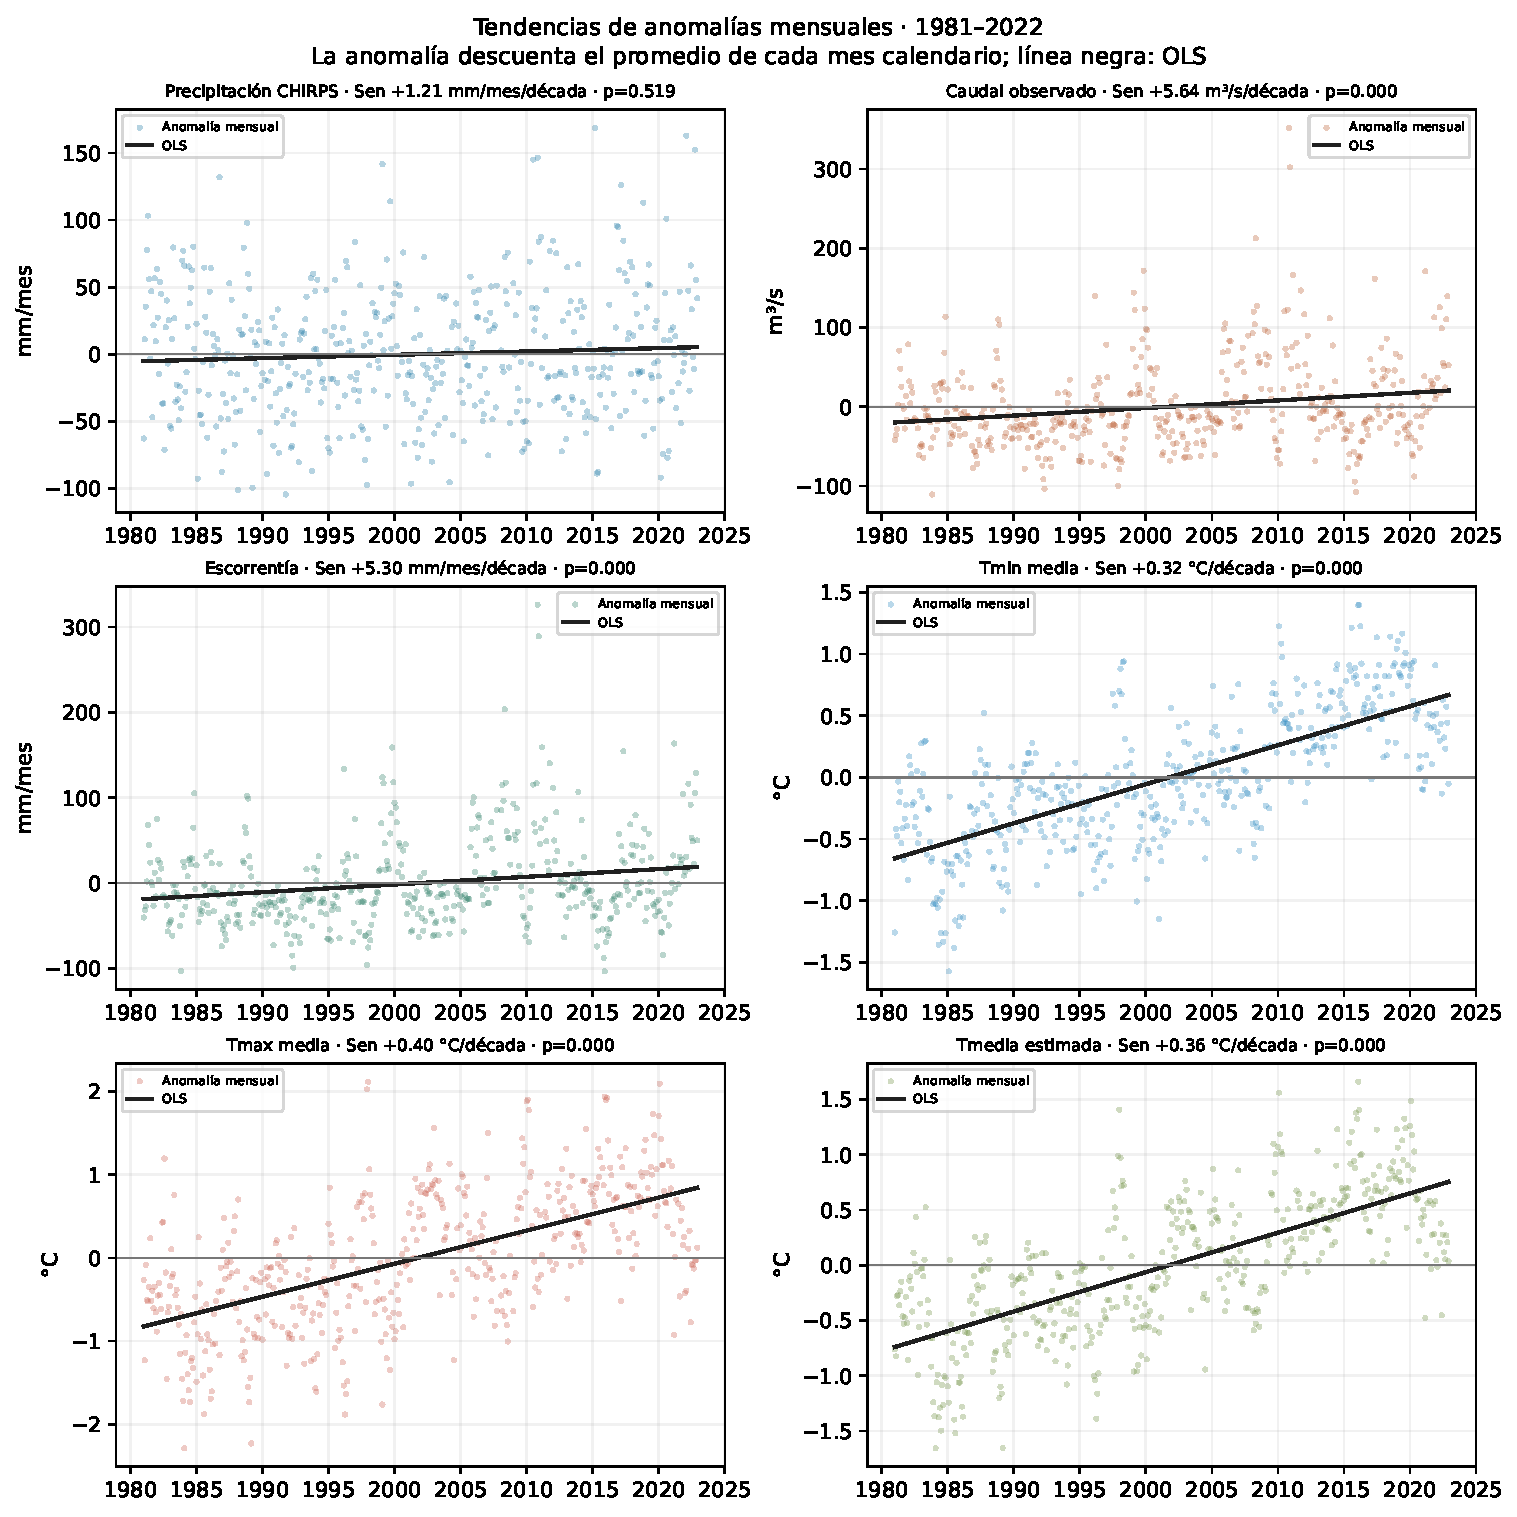
\includegraphics[width=\linewidth]{figuras/tendencias_mensuales.pdf}
\caption{Anomalías mensuales y recta OLS, 1981--2022. Los títulos presentan la pendiente de Sen estacional por década y el valor p de Mann--Kendall estacional.}
\end{figure}

\begin{center}\small
\begin{tabular}{lrrrr}\hline
Variable & OLS/década & Sen/década & p & Significativa 5\% \\ \hline
Precipitación CHIRPS & 2,50 & 1,21 & 0,519 & no \\
Caudal observado & 9,59 & 5,64 & 0,000 & sí \\
Escorrentía & 9,02 & 5,30 & 0,000 & sí \\
Tmin media & 0,32 & 0,32 & 0,000 & sí \\
Tmax media & 0,40 & 0,40 & 0,000 & sí \\
Tmedia estimada & 0,36 & 0,36 & 0,000 & sí \\
\hline\end{tabular}
\end{center}

\subsection*{Lectura de los resultados}
\begin{itemize}
\item Precipitación CHIRPS: Sen estacional 1,21 mm/mes/década; p=0,519. no hay evidencia estadística de una tendencia monotónica al 5 \% (aumento).
\item Caudal observado: Sen estacional 5,64 m$^3$/s/década; p=0,000. hay evidencia estadística de una tendencia monotónica al 5 \% (aumento).
\item Escorrentía: Sen estacional 5,30 mm/mes/década; p=0,000. hay evidencia estadística de una tendencia monotónica al 5 \% (aumento).
\item Tmin media: Sen estacional 0,32 $^\circ$C/década; p=0,000. hay evidencia estadística de una tendencia monotónica al 5 \% (aumento).
\item Tmax media: Sen estacional 0,40 $^\circ$C/década; p=0,000. hay evidencia estadística de una tendencia monotónica al 5 \% (aumento).
\item Tmedia estimada: Sen estacional 0,36 $^\circ$C/década; p=0,000. hay evidencia estadística de una tendencia monotónica al 5 \% (aumento).
\end{itemize}
R se deriva directamente de Q, por lo que sus resultados no son evidencias
independientes. Tmedia se estima como $(Tmin+Tmax)/2$ y tampoco es una
observación independiente. IMERG no entra al análisis: aún no se cuenta con
valores mensuales descargados y verificados.
